% This is samplepaper.tex, a sample chapter demonstrating the
% LLNCS macro package for Springer Computer Science proceedings;
% Version 2.20 of 2017/10/04
%
\documentclass[runningheads]{llncs}
%
\usepackage{graphicx}
% Used for displaying a sample figure. If possible, figure files should
% be included in EPS format.
%
% If you use the hyperref package, please uncomment the following line
% to display URLs in blue roman font according to Springer's eBook style:
% \renewcommand\UrlFont{\color{blue}\rmfamily}
\usepackage{listings}
\usepackage{xcolor}
\usepackage[T1]{fontenc}
\usepackage{minted}
\definecolor{backcolour}{rgb}{0.95,0.95,0.92} 
\lstdefinestyle{code}{
    backgroundcolor=\color{backcolour}, % colour for the background. External color or xcolor package needed.
    basicstyle=\ttfamily\footnotesize,  % font size/family/etc. for source (e.g. basicstyle=\ttfamily\small)
    breaklines=true,                    % automatic line-breaking
    captionpos=b,                       % position of caption (t/b)
    keepspaces=true,                    %  keep spaces in the code, useful for indetation
    numbers=left,                       % position of line numbers (left/right/none, i.e. no line numbers)
    numbersep=5pt,                      % distance of line-numbers from the code
    showspaces=false,                   % emphasize spaces in code (true/false)
    showstringspaces=false,             % emphasize spaces in strings (true/false)
    showtabs=false,                     % emphasize tabulators in code (true/false)  
    tabsize=2                           % default tabsize
    }
    
\lstdefinelanguage{Dockerfile}
{
  morekeywords={FROM, RUN, CMD, LABEL, MAINTAINER, EXPOSE, ENV, ADD, COPY,
    ENTRYPOINT, VOLUME, USER, WORKDIR, ARG, ONBUILD, STOPSIGNAL, HEALTHCHECK,
    SHELL},
  morecomment=[l]{\#},
  morestring=[b]"
}

\lstset{style=code}
\lstset{
    columns=flexible,
    keepspaces=true,
    showstringspaces=false,
    basicstyle=\ttfamily\footnotesize,  % font size/family/etc. for source (e.g. basicstyle=\ttfamily\small)
    commentstyle=\color{gray},
    keywordstyle=\color{purple},
    stringstyle=\color{green}
}
\begin{document}
%
\title{Cloud Computing Systems Second Work Report}
%
%\titlerunning{Abbreviated paper title}
% If the paper title is too long for the running head, you can set
% an abbreviated paper title here
%
\author{Diogo Almeida\inst{58369} \and
Diogo Fona\inst{57940} \and
Bruno Cabrita\inst{57833}}
%
\authorrunning{D. Almeida, D. Fona and B. Cabrita}
% First names are abbreviated in the running head.
% If there are more than two authors, 'et al.' is used.
%
\institute{NOVA School of Science and Technology - MSc in Computer Engineering 
\email{\{brm.cabrita,daro.almeida,d.fona\}@campus.fct.unl.pt}}
%
\maketitle % typeset the header of the contribution
%
\section{Assignment Solution}

In this work, we implement the application presented in the first work and deploy it in Azure in a Kubernetes cluster, instead of using the built-in Azure components. To achieve this we build containers, using Docker, with the application's constituents and deploy them in Kubernetes Pods. 

%  implement project1 application in Azure with Kubernetes and different technology 

\subsection{Implementation}

As in the previous work, for the application to support the storage, querying, and processing of information, we use cloud software and hardware components that we deploy with Kubernetes: (settings described in deployment files in appendix)

\subsubsection{Application:}

The application's backend that was implemented in the first work is built in a container and deployed. Since we use different components the communication API calls with them are altered. The application is accessed externally its a LoadBalancer type service.

\subsubsection{Database:}

The database we use is MongoDB instead of Azure CosmosDB. Particularly in this work for simplicity its information is not stored persistently.

\subsubsection{Media Storage:}

For the storage of media content in the application we use a Persistent Volume Claim instead of Azure Blob Storage. It stores the contents persistently in a file system volume.

\subsubsection{Cache:}

The caching system we use is Redis like in the first work.

\subsubsection{Serverless Functions:}

Regarding serverless functions that were previously implemented with Azure Functions, functions that were timer based (TimerTrigger) are implemented with CronJobs, and the rest in separate deployments.

\subsubsection{Message Queues:}

The message queue system we use is RabbitMQ instead of Azure Service Bus.

\subsection{Pods}

Each of the Kubernetes cluster's Pods are single-container and contain the application's services: backend, mongodb, rabbitmq, redis, and one for each function.

\section{Evaluation}

\begin{figure}
    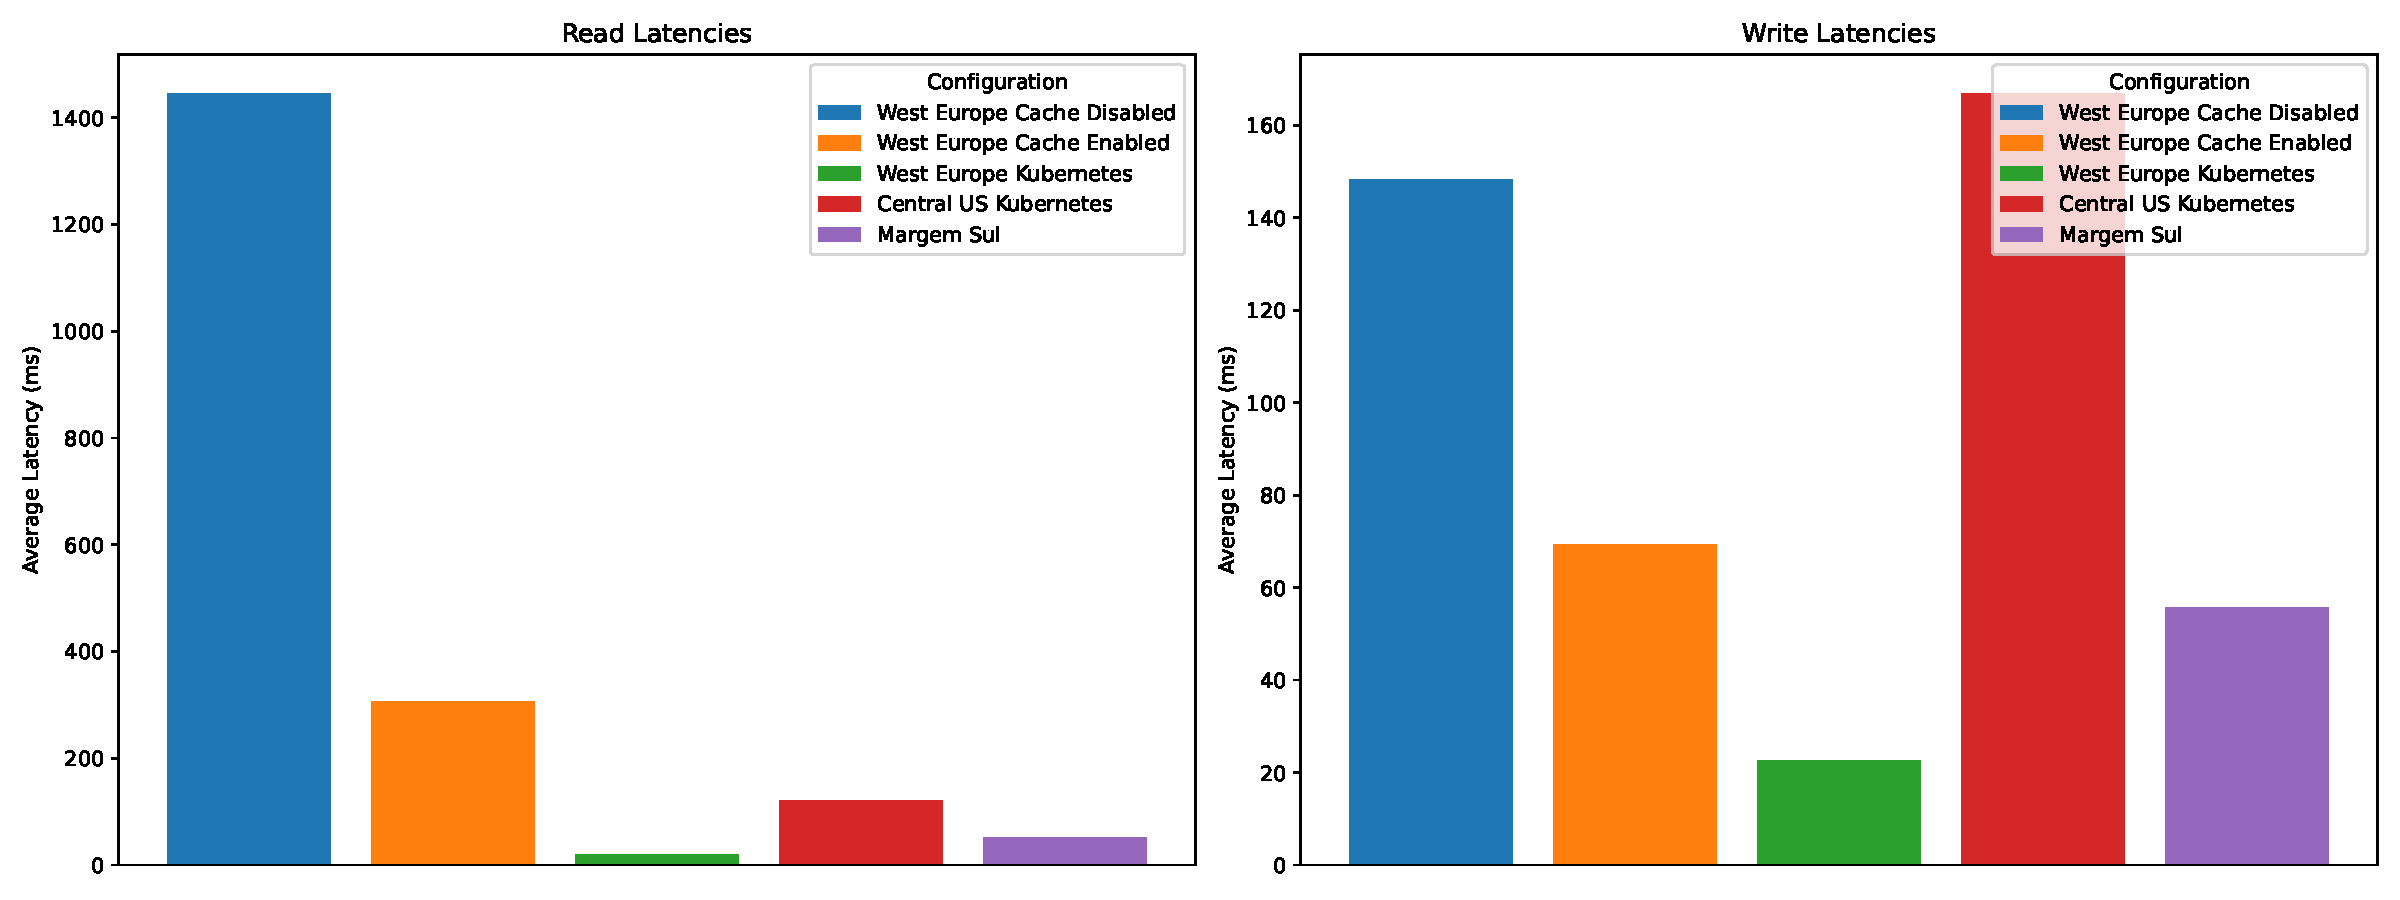
\includegraphics[width=\textwidth]{latencies}
    \caption{Average latency in milliseconds of read and write operations from clients in different regions with the application in West Europe. The blue bar concerns the previous implementation that used Azure services and the remaining concerns the new one that uses the Kubernetes cluster.} \label{fig:latencies}
\end{figure}

To perform the evaluation of our implementation we deploy a Docker container with workload tests executed with Artillery, using Azure Container Instances, in different regions and also run it locally with Docker.

The results shown in Fig.~\ref{fig:latencies} demonstrate that using either the Azure services or Kubernetes with alternate services has no significant difference in impact. 

In the graph of writes it's observed that using Kubernetes perceives slightly lower latency but that is probably due to the different mechanism's performance or variance.  

In the graph of reads we can see that the previous implementation has a much higher perceived latency. This is because we repaired an implementation issue that caused some listing operations to make too much requests which we mentioned in the first work.

\clearpage
\appendix
\section{Dockerfiles}

\begin{lstlisting}[language=Dockerfile, caption=backend.dockerfile]
FROM docker.io/tomcat:10-jdk17-corretto
WORKDIR /usr/local/tomcat/webapps
RUN curl https://github.com/open-telemetry/opentelemetry-java-instrumentation/releases/download/v1.20.2/opentelemetry-javaagent.jar -L --output opentelemetry-javaagent.jar
ENV JAVA_OPTS="-ea -javaagent:opentelemetry-javaagent.jar"
COPY modules/backend-app/target/scc-backend-app-1.0-SNAPSHOT.war ROOT.war
EXPOSE 8080
\end{lstlisting}

\begin{lstlisting}[language=Dockerfile, caption=worker.dockerfile]
FROM docker.io/amazoncorretto:19
WORKDIR /usr/local/app
ENV JAVA_OPTS="-ea"
COPY modules/worker-assembly/target/scc-worker-assembly-1.0-SNAPSHOT-jar-with-dependencies.jar app.jar
ENTRYPOINT ["java", "-cp", "app.jar"]
\end{lstlisting}

\begin{lstlisting}[language=Dockerfile, caption=tester.dockerfile]
FROM docker.io/artilleryio/artillery
WORKDIR /usr/local/app
RUN npm install @faker-js/faker --save-dev
ADD tester/testing/artillery/*.yml .
ADD tester/testing/artillery/*.js .
COPY tester/artillery-entrypoint.sh .
ENTRYPOINT ["/bin/sh", "./artillery-entrypoint.sh"]
\end{lstlisting}

\section{Kubernetes deployment files}

\subsubsection{backend.yaml}
\begin{minted}[
    gobble=4,
    frame=single,
    linenos,
    breaklines 
  ]{yaml}
    apiVersion: v1
    kind: ConfigMap
    metadata:
      name: scc-backend-cmap
    data:
      KUBE_CACHING_ENABLED: "true"
      KUBE_MEDIA_DATA_DIRECTORY: /var/data
      KUBE_MONGO_CONNECTION_URI: mongodb://scc-mongodb:27017
      KUBE_MONGO_DATABASE_NAME: scc-backend
      KUBE_MONGO_AUCTION_COLLECTION: auctions
      KUBE_MONGO_BID_COLLECTION: bids
      KUBE_MONGO_QUESTION_COLLECTION: questions
      KUBE_MONGO_USER_COLLECTION: users
      KUBE_REDIS_URL: scc-redis
      KUBE_REDIS_PORT: "6379"
      KUBE_RABBITMQ_HOST: scc-rabbitmq
      KUBE_OTLP_ENABLED: "true"
      KUBE_RABBITMQ_PORT: "5672"
    ---
    apiVersion: v1
    kind: PersistentVolumeClaim
    metadata:
      name: scc-backend-pvc
    spec:
      resources:
        requests:
          storage: 2Gi
      storageClassName: azurefile
      volumeMode: Filesystem
      accessModes:
        - ReadWriteOnce
    
    ---
    apiVersion: apps/v1
    kind: Deployment
    metadata:
      name: scc-backend
    spec:
      selector:
        matchLabels:
          app: scc-backend
      template:
        metadata:
          labels:
            app: scc-backend
        spec:
          containers:
            - name: scc-backend
              image: git.d464.sh/diogo464/scc-backend
              resources:
                limits:
                  memory: "1Gi"
                  cpu: "500m"
              ports:
                - containerPort: 8080
              volumeMounts:
                - mountPath: /var/data
                  name: scc-backend-pvc
              envFrom:
                - configMapRef:
                    name: scc-backend-cmap
          volumes:
            - name: scc-backend-pvc
              persistentVolumeClaim:
                claimName: scc-backend-pvc
    ---
    apiVersion: v1
    kind: Service
    metadata:
      name: scc-backend
    spec:
      type: LoadBalancer
      selector:
        app: scc-backend
      ports:
        - port: 80
          targetPort: 8080
    ---
    apiVersion: apps/v1
    kind: Deployment
    metadata:
      name: scc-worker-auction-close
    spec:
      selector:
        matchLabels:
          app: scc-worker-auction-close
      template:
        metadata:
          labels:
            app: scc-worker-auction-close
        spec:
          containers:
            - name: scc-worker-auction-close
              image: git.d464.sh/diogo464/scc-worker
              args: [scc.worker.AuctionClose]
              resources:
                limits:
                  memory: "128Mi"
                  cpu: "80m"
              envFrom:
                - configMapRef:
                    name: scc-backend-cmap
    ---
    apiVersion: apps/v1
    kind: Deployment
    metadata:
      name: scc-worker-auction-popularity-consumer
    spec:
      selector:
        matchLabels:
          app: scc-worker-auction-popularity-consumer
      template:
        metadata:
          labels:
            app: scc-worker-auction-popularity-consumer
        spec:
          containers:
            - name: scc-worker-auction-popularity-consumer
              image: git.d464.sh/diogo464/scc-worker
              args: [scc.worker.AuctionPopularityConsumer]
              resources:
                limits:
                  memory: "128Mi"
                  cpu: "50m"
              envFrom:
                - configMapRef:
                    name: scc-backend-cmap
    ---
    apiVersion: batch/v1
    kind: CronJob
    metadata:
      name: scc-worker-auction-popularity-updater
    spec:
      schedule: "*/1 * * * *"
      jobTemplate:
        spec:
          template:
            spec:
              containers:
                - name: scc-worker-auction-popularity-updater
                  image: git.d464.sh/diogo464/scc-worker
                  args: [scc.worker.AuctionPopularityUpdater]
                  resources:
                    limits:
                      memory: "128Mi"
                      cpu: "80m"
                  envFrom:
                    - configMapRef:
                        name: scc-backend-cmap
              restartPolicy: OnFailure
\end{minted}


\subsubsection{mongo.yaml}
\begin{minted}[
    gobble=4,
    frame=single,
    linenos,
    breaklines
  ]{yaml}
    apiVersion: apps/v1
    kind: Deployment
    metadata:
      name: scc-mongodb
    spec:
      selector:
        matchLabels:
          app: scc-mongodb
      strategy:
        type: Recreate
      template:
        metadata:
          labels:
            app: scc-mongodb
        spec:
          containers:
            - name: scc-mongodb
              image: docker.io/mongo:5.0.14
              resources:
                limits:
                  memory: "256Mi"
                  cpu: "500m"
              ports:
                - containerPort: 27017
    ---
    apiVersion: v1
    kind: Service
    metadata:
      name: scc-mongodb
    spec:
      selector:
        app: scc-mongodb
      ports:
        - port: 27017
    
\end{minted}

\subsubsection{rabbitmq.yaml}
\begin{minted}[
    gobble=4,
    frame=single,
    linenos,
    breaklines
  ]{yaml}
    apiVersion: v1
    kind: ConfigMap
    metadata:
      name: scc-rabbitmq-cmap
    data:
      config: ""
      plugins: |
        [rabbitmq_management,rabbitmq_management_agent].
    ---
    apiVersion: v1
    kind: ConfigMap
    metadata:
      name: scc-rabbitmq-cmap-env
    data:
      RABBITMQ_ENABLED_PLUGINS_FILE: /usr/local/configs/enabled_plugins
      #RABBITMQ_CONFIG_FILE: /usr/local/configs/rabbitmq
    ---
    apiVersion: apps/v1
    kind: Deployment
    metadata:
      name: scc-rabbitmq
    spec:
      selector:
        matchLabels:
          app: scc-rabbitmq
      template:
        metadata:
          labels:
            app: scc-rabbitmq
        spec:
          containers:
            - name: scc-rabbitmq
              image: rabbitmq
              resources:
                limits:
                  memory: "196Mi"
                  cpu: "500m"
              ports:
                - containerPort: 5672
                - containerPort: 15672
              volumeMounts:
                - mountPath: /usr/local/configs
                  name: scc-rabbitmq-config-vol
              envFrom:
                - configMapRef:
                    name: scc-rabbitmq-cmap-env
          volumes:
            - name: scc-rabbitmq-config-vol
              configMap:
                name: scc-rabbitmq-cmap
                items:
                  - key: config
                    path: rabbitmq.config
                  - key: plugins
                    path: enabled_plugins
    ---
    apiVersion: v1
    kind: Service
    metadata:
      name: scc-rabbitmq
    spec:
      selector:
        app: scc-rabbitmq
      ports:
        - port: 5672
    
\end{minted}

\subsubsection{redis.yaml}
\begin{minted}[
    gobble=4,
    frame=single,
    linenos,
    breaklines
  ]{yaml}
    apiVersion: apps/v1
    kind: Deployment
    metadata:
      name: scc-redis
    spec:
      selector:
        matchLabels:
          app: scc-redis
      template:
        metadata:
          labels:
            app: scc-redis
        spec:
          containers:
            - name: scc-redis
              image: docker.io/redis:7.0.5
              resources:
                limits:
                  memory: "256Mi"
                  cpu: "500m"
              ports:
                - containerPort: 6379
    ---
    apiVersion: v1
    kind: Service
    metadata:
      name: scc-redis
    spec:
      selector:
        app: scc-redis
      ports:
        - port: 6379
\end{minted}

\end{document}
